\documentclass[12pt]{article}
\usepackage{amsmath}
\usepackage{graphicx,psfrag,epsf}
\usepackage{enumerate}
\usepackage{natbib}
\usepackage{textcomp}
\usepackage[hyphens]{url} % not crucial - just used below for the URL
\usepackage{hyperref}
\providecommand{\tightlist}{%
  \setlength{\itemsep}{0pt}\setlength{\parskip}{0pt}}

%\pdfminorversion=4
% NOTE: To produce blinded version, replace "0" with "1" below.
\newcommand{\blind}{0}

% DON'T change margins - should be 1 inch all around.
\addtolength{\oddsidemargin}{-.5in}%
\addtolength{\evensidemargin}{-.5in}%
\addtolength{\textwidth}{1in}%
\addtolength{\textheight}{1.3in}%
\addtolength{\topmargin}{-.8in}%

%% load any required packages here



% Pandoc citation processing

\usepackage{pdflscape}

\begin{document}


\def\spacingset#1{\renewcommand{\baselinestretch}%
{#1}\small\normalsize} \spacingset{1}


%%%%%%%%%%%%%%%%%%%%%%%%%%%%%%%%%%%%%%%%%%%%%%%%%%%%%%%%%%%%%%%%%%%%%%%%%%%%%%

\if0\blind
{
  \title{\bf ``A p-value of $<$ 0.05 was considered statistically significant'': a content analysis of published statistical methods sections}

  \author{
        Nicole M White \thanks{The authors gratefully acknowledge computational resources and services
used in this work provided by the eResearch Office, Queensland
University of Technology, Brisbane, Australia.} \\
    \small{Australian Centre for Health Services Innovation and Centre for Healthcare Transformation} \\
\small{School of Public Health and Social Work, Queensland University of Technology} \\
     and \\     Thiru Balasubramaniam, Richi Nayak \\
    \small{Centre for Data Science and School of Computer Science} \\
\small{Queensland University of Technology} \\
     and \\     Adrian G Barnett \\
    \small{Australian Centre for Health Services Innovation and Centre for Healthcare Transformation} \\
\small{School of Public Health and Social Work, Queensland University of Technology} \\
      }
  \maketitle
} \fi

\if1\blind
{
  \bigskip
  \bigskip
  \bigskip
  \begin{center}
    {\LARGE\bf ``A p-value of $<$ 0.05 was considered statistically significant'': a textual analysis of published statistical methods sections}
  \end{center}
  \medskip
} \fi

\bigskip
\begin{abstract}
The text of your abstract. 200 or fewer words.
\end{abstract}

\noindent%
{\it Keywords:} 3 to 6 keywords, that do not appear in the title
\vfill

\newpage
\spacingset{1.45} % DON'T change the spacing!

\hypertarget{introduction}{%
\section{Introduction}\label{introduction}}

An ideal statistical analysis will use appropriate methods to create
insights from the data and inform the research questions. Unfortunately
many current statistical analyses are far from ideal, with many
researchers using the wrong methods, misinterpreting the results, or
failing to adequately check their assumptions \citep{2008, Leek2017}.
Some researchers take a ``mechanistic'' approach to statistics, copying
the few methods they know regardless of their appropriateness, and then
going through the motions of the analysis \citep{Stark2018}. 

Many researchers lack adequate training in research methods, and
statistics is something they do with trepidation and even ignorance
\citep{Altman1994, King2019}. However, using the wrong statistical
methods can cause real harm \citep{Altman1994, Brown2018} and bad
statistical practices are being to used abet weak science
\citep{Stark2018}. Statistical mistakes are a key source of waste in
research and partly explain the current reproducibility crisis in
science \citep{Allison2016}. Even when the correct methods are used,
many researchers fail to describe them adequately, making it difficult
to reproduce the results \citep{Ernst2017, Zhou2018}. Poor statistical
methods might not be caught by reviewers, as they may not be qualified
to judge the statistics. A recent survey of editors found that only 23\%
of health and medical journals used expert statistical review for all
articles \citep{Hardwicke2020}, which was little different from a survey
from 22 years ago \citep{Goodman1998}.

There is guidance for researchers on how to write up their statistical
methods and results. The International Committee of Medical Journal
Editors recommend that researchers should: ``Describe statistical
methods with enough detail to enable a knowledgeable reader with access
to the original data to judge its appropriateness for the study and to
verify the reported results'' \citep{ICMJE2019}. More detailed guideance
is given by the SAMPL and EQUATOR guidelines
\citep{Lang2013, Altman2016} with the latter covering all apsects of the
paper. Both of these guidelines were led by Doug Altman, who spoke often
and for many years about the need for better statistical reporting. The
awareness and use of these guidelines could be improved. There were 256
Google Scholar citations to the SAMPL paper (as at 15 March 2021) which
is a good citation statistic for most papers, but is low considering the
millions of papers that use statistical analysis.

A potential contributor to poor statistical reporting is the temptation for researchers to re-use
descriptions of statistical methods, in an effort to make their papers resemble those of their peers 
and increase perceived chances of publication  \citep{Diong2018}. Two statisticians on this paper 
(AB and NW) have heard researchers admit
that they have copied-and-pasted their statistical methods sections from
other papers, regardless of whether they are appropriate. For this paper, we applied a text-based 
clustering method to analyse the content of published statistical methods sections.
Clustering results are then evaluated to estimate the extent that researchers are
using cut-and-paste or `boilerplate' statistical methods sections.
Boilerplate text is that ``which can be reused in new contexts or
applications without significant changes to the original''
\citep{Wikipedia}. Use of these methods sections indicates that little
thought has gone into the statistical analysis.

\hypertarget{methods}{%
\section{Methods}\label{methods}}

\subsection{Data sources}

We used two openly available data sources to find statistical methods
sections: research articles published in \emph{PLOS ONE} and study
protocols registered on the Australian and New Zealand Clinical Trials
Registry (ANZCTR). Data sources were chosen as examples of common
research outputs that include descriptions of statistical methods that
were used, or are planned, for analysing study outcomes.

\subsubsection{Public Library of Science (PLOS ONE)}
\label{sec:methodsPLOS}

\emph{PLOS ONE} is a open access mega-journal that publishes original
research across a wide range of scientific fields. Article submissions
are handled by an academic editor who selects peer reviewers based on
their self-nominated areas of expertise. Currently there are 324 academic editors out of 9,648 (3\%) 
with the keywords of "statistics (mathematics)" or "statistical methods" in their expertise list (web search on 25-May-2021,
 https://journals.plos.org/plosone/static/editorial-board). Submissions do not undergo
formal statistical review. Instead, reviewers are required to assess
submissions against several publication criteria, including whether:
``Experiments, statistics, and other analyses are performed to a high
technical standard and are described in sufficient detail''
\citep{PLOS}. All reviewers are asked the question: ``Has the
statistical analysis been performed appropriately and rigorously?'',
with the possible responses of ``Yes'', ``No'' and ``I don't know''.

Authors are encouraged to follow published reporting guidelines such as
EQUATOR, to ensure that chosen statistical methods are appropriate for
the study design, and adequate details are provided to enable
independent replication of results.

All \emph{PLOS ONE} articles are freely accessible via the PLOS
Application Programming Interface (API). This enabled us to conduct
searches of full-text articles and analyse data on articles' text
content and general attributes such as publication date and field(s) of
research. Statistical methods sections were extracted using a two-step
approach:

\emph{Step 1}: Targeted API searches were completed using the R package
`rplos' \citep{rplos}. Search queries targeted analysis-related terms,
combining the words ``data'' or ``statistical'' with one of:
``analysis'', ``analyses'', ``method'', ``methodology'' or
``model(l)ing''. Terms could appear anywhere within the main body of the
article, to account for the placement of relevant text in different
sections, for example, in the \emph{Material and Methods} section versus
\emph{Results}. Search results were indexed by a unique Digital Object
Identifier (DOI). Attribute data collected per DOI included journal
volume and subject classification(s).

\emph{Step 2}: \emph{PLOS ONE} does not prescribe standardised headings
to preface statistical methods sections. To address this, we performed
partial matching on available headings against frequently used terms in
initial search results: `Statistical analysis', `Statistical analyses',
`Statistical method', `Statistics', `Data analysis' and `Data analyses'.

Data were downloaded on 3 July 2020. For
records that did not pass Step 2, we reviewed where initial search terms
appeared in the full-text, to determine the proportion of
statistical methods sections that were missed under our chosen approach.

\subsubsection{Australia and New Zealand Clinical Trials Registry (ANZCTR)}
\label{sec:methodsANZCTR}

The ANZCTR was established in 2005 as part of a coordinated global
effort to improve research quality and transparency in clinical trials
reporting; observational studies can also be registered. All studies
registered on ANZCTR are publicly available and can be searched via an
online portal (\url{https://www.anzctr.org.au}).

Details required for registration follow a standardised template
\citep{ANZCTR}, which covers participant eligibility, the
intervention(s) being evaluated, study design and outcomes. The
information provided must be in English. Studies are not peer reviewed.

For the statistical methods section, researchers are asked to provide a
``brief description'' of the sample size calculations, statistical
methods and planned analyses, although this section is not compulsory
\citep{ANZCTR}. Studies are reviewed by ANZCTR staff for completeness of
key information, which does not include the completeness of the
statistical methods sections.

All studies available on ANZCTR were downloaded on 1 February 2020 in
XML format. We used all the text available in the ``Statistical
methods'' section. We also collated basic information about the study
including the study type (interventional or observational), submission
date, number of funders and target sample size. These variables were
chosen as we believed they might influence the completeness of the
statistical methods section, because we expected larger studies and
those with funding to be more complete, and we also were interested in
changes over time.

Studies prior to 2013 were excluded as the statistical methods section
appeared to be introduced in 2013. Some studies were first registered on
the alternative trial database \emph{clinicaltrials.gov} and then also
posted to ANZCTR. We excluded these studies because they almost all had
no completed statistical methods section as this section is not included
in \emph{clinicaltrials.gov}.

Statistical methods sections were missing for some studies downloaded
from ANZCTR, including sections labelled as ``Not
applicable'', ``Nil'' or ``None''. We examined if there were
particular studies where the statistical methods section was more likely to be missing.
Analysis considered a logistic regression model estimated in the
Bayesian framework {[}\citet{INLA}; www.r-inla.org{]}, with missing
statistical methods section (yes/no) as the dependent variable. The independent variables were date,
study type (observational or interventional), number of funders and
target sample size. Results were
reported as odds ratios with 95\% credible intervals (CI).

\subsection{Full-text processing}
\label{sec:methods-cleaning}

Text cleaning aimed to standardise notation and statistical terminology,
whilst minimising changes to article style and formatting. \emph{R} code
used for data extraction and cleaning is available from
\url{https://github.com/agbarnett/stats_section}.

Mathematical notation was converted from Unicode characters to plain
text. For example, the Unicode character corresponding to \(\theta\)
(\textless U+03B8\textgreater) was replaced with `theta'. Common symbols
outside of Unicode blocks including `\%' (percent) and `\textless{}'
(`less-than') were similarly converted into plain text. General
formatting was removed, including carriage returns, punctuation marks,
in-text references (e.g.~``{[}42{]}'') centred equations, and other
non-ASCII characters. Text contained inside brackets was retained to
maximise content for analysis, with brackets removed. Common stop words
including pronouns, contractions and selected prepositions were removed.
We retained selected stop words that, if excluded, may have changed the
context of statistical methods being described, for example `between'
and `against'.

We compiled an extensive list of statistical terms to standardise
reported descriptions of statistical methods. An initial list was
compiled by calculating individual word frequencies and identifying
relevant terms that appeared at least 100 times. Further terms were
sourced from index searches of three statistics textbooks
\citep{Diggle2013,Bland2015,Dobson2018}. Plurals (e.g.,
`chi-squares') unhyphenated (e.g., `chi square') and combined
(e.g.~`chisquare') terms were transformed to singular, hyphenated form
(e.g., `chi-square'). Common statistical tests were also hyphenated
(e.g., `hosmer lemeshow' to `hosmer-lemeshow'). The final list is
provided in Supplementary File 1.

\subsection{Clustering algorithm}

Text from statistical methods sections was analysed using Non-Negative
Matrix Factorization (NMF). NMF is an established approach for topic
modelling, and provides an effective solution for text-based clustering
when dealing with high-dimensional data
\citep[\citet{luong2019clustering}]{kim2014algorithms}. In this section,
we outline key details of NMF and its strengths compared with other
text-based clustering methods.

For \(N\) studies, let \(P \in R^{M \times N}\) denote a content matrix of text from statistical methods sections as \(M\) unique
terms. Text clustering algorithms for identifying common topics across
studies requires \(P\) to be represented with a vector space model. In
our case, unique terms in \(P\) are modelled using the tf-idf (term
frequency \(\times\) inverse document frequency) weighting schema, to
account for the relative importance of common and rare terms.

A common problem facing text clustering algorithms is the curse of
dimensionality due to the high number of terms in the doc\(\times\)term
matrix representation
\citep[\citet{sutanto2018fine}]{aggarwal2012mining}. Applying text-based
methods based on distance, density or probability therefore face
difficulties in high-dimensional settings
\citep[\citet{mohotti2018corpus},\citet{mohotti2019concept}]{park2018examining}.
Specifically, distances between near and far points becomes negligible
\citep{aggarwal2012mining}. This behaviour directly affects the
performance of distance-based clustering methods such as
\textit{k}-means \citep{jain2010} in accurately identifying subgroups
(topics) present in the data. Furthermore, sparseness associated with
high-dimensional matrix representations does not allow for
differentiation between topics based on density differences
\citep[\citet{mohotti2018efficient}]{mohotti2018corpus}.

To address these limitations, NMF deals with high-dimensional data by
mapping it to a lower-dimensional space. This mapping this achieved by
approximating \(P\) with two factor matrices: \(W \in R^{M \times g}\)
and \(H \in R ^{N \times g}\) \citep{aggarwal2012mining}, such that
\(P \approx WH^{T}\). The number of subgroups of common topic inferred
from the data is given by \(g\).

The matrix factorization process approximates the lower dimensional
non-negative factor matrices \(W\) and \(H\) such that they can
represent high dimensional \(P\) with the least error. Estimation of
\(W\) and \(H\) is achieved by optimising an objective function; for
NMB, the Fronbeius norm is used, equivalent to minimising the sum of
squares for all elements of \(P\):

\begin{equation}
\label{eq:NMFobjectivefn}
\min \frac{1}{2}\|P - WH\|= \sum _{i=1}^{M}\sum _{j=1}^{N} \left(  P_{i,j} -\left(WH \right)_{i,j} \right)^{2}
\end{equation}

Following estimation, \textit{H} contains the information regarding
topic membership for all studies. In our case, topic membership
\((1,\ldots,g)\) for a statistical methods section is inferred from the
maximum coefficient value in the corresponding row of \(H\), also known
as the topic coherence score. For our two datasets, we applied NMF with
\(g=10\) topics.

\subsection{Content analysis}

Clustering results were visualised by word clouds to summarise
frequently occurring terms associated with topic membership. Whilst
these results were useful for inferring common themes across statistical
methods sections, they did not indicate evidence of boilerplate text
beyond the use of common terms. Follow up analysis therefore considered
similarities in text between sections assigned to the same topic.

We used the Jaccard similarity index to compare the statistical methods
section with the highest topic coherence score with all other sections
assigned to the same topic. Indices were calculated at the sentence
level, to account for instances of boilerplate text within larger
methods sections. We chose the Jaccard index as an easy to interpret
measure, which summarises the similarity between two sentences by the
number of words common to each sentence (intersection), divided by the
number of words that appeared in either sentence (union). Instances of
boilerplate text were defined by a Jaccard index of 0.9 or higher and a
difference in word count of plus or minus three words.

\clearpage

\section{Results}\label{results}

\subsection{PLOS ONE}\label{plos-one}

API searches returned 131,847 papers (DOIs)
(\autoref{fig:consort-diagrams}). After partial matching, 111,731 (85\%)
statistical methods sections were identified. In the final sample,
95,518 (85\%) DOIs returned an exact match against common section
headings: 64,133 for `statistical analysis', 13,380 for `statistical
analyses' and 13,627 for `data analysis'.

\begin{figure}[htbp]

{\centering 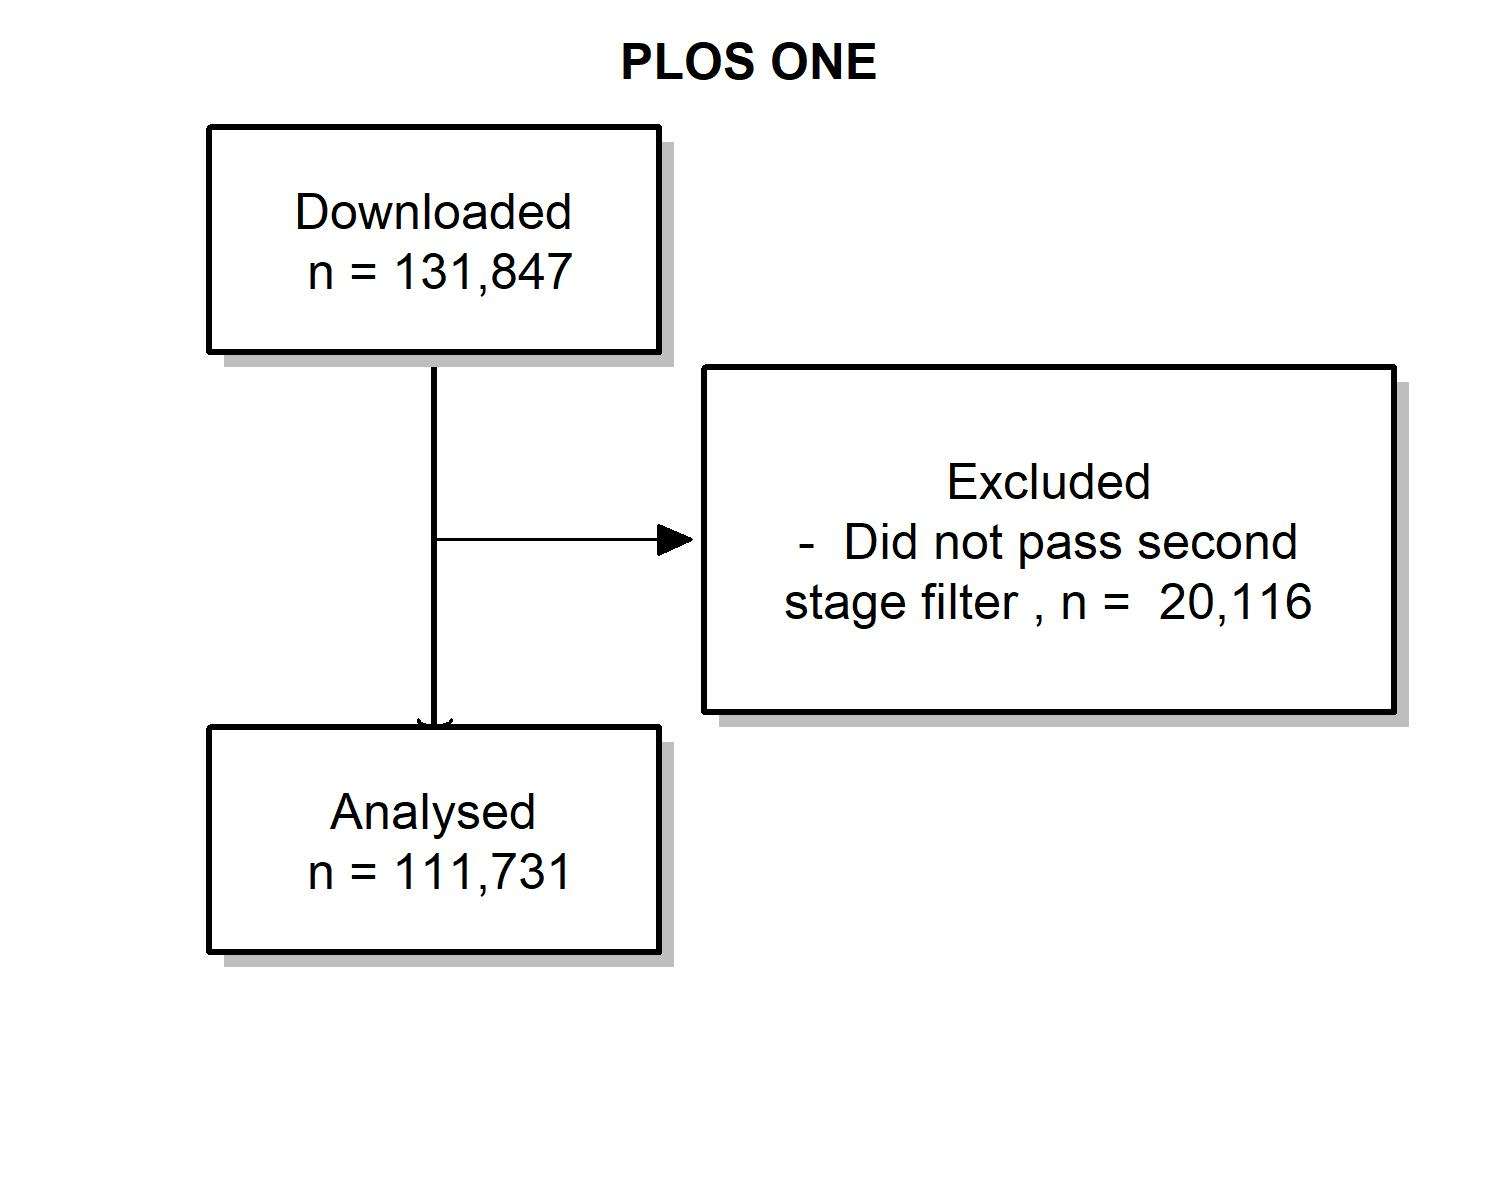
\includegraphics[width=0.49\linewidth]{figures/excluded_plosone} 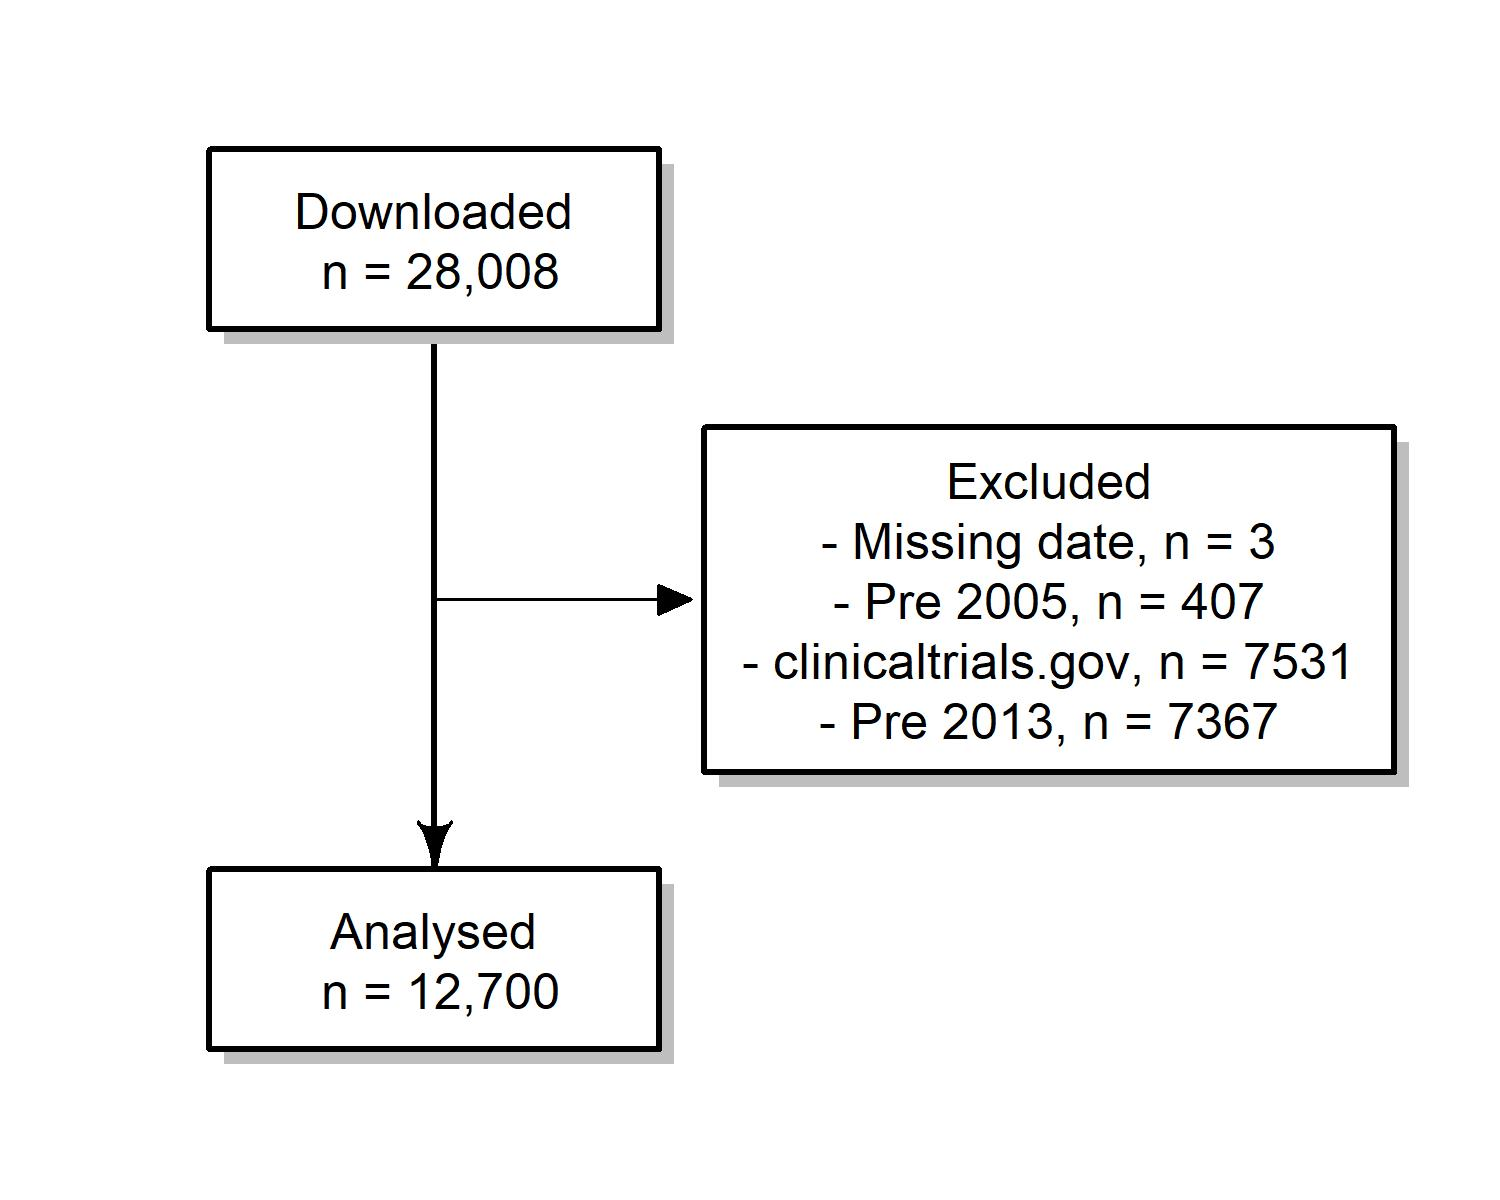
\includegraphics[width=0.49\linewidth]{figures/excluded_anzctr_missing} 

}

\caption{\label{fig:consort-diagrams}Search results for PLOS ONE (left) and ANZCTR (right).}
\end{figure}

\begin{figure}[htbp]

{\centering 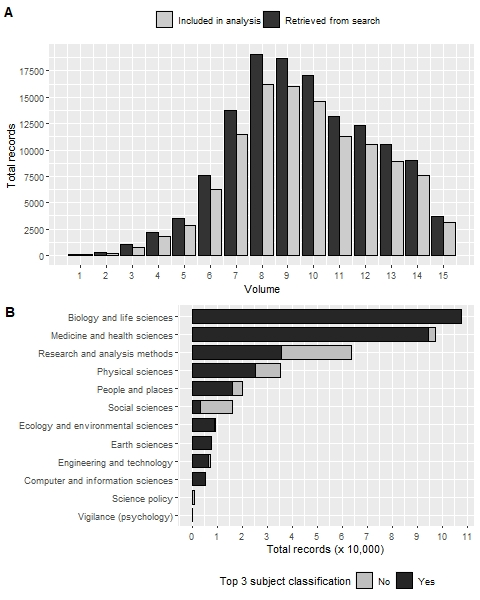
\includegraphics[width=0.6\linewidth]{figures/plos_summary} 

}

\caption{\label{fig:plos-n} A: Search results by PLOS ONE volume; B: Subject classifications assigned to full-text recorded included in the analysis}
\end{figure}

Search results varied by journal volume (Figure \ref{fig:plos-n}A). The
total number of API search results peaked at volumes 8 (n = 19,045) and
9 (n = 19,045) in years 2013 and 2014. This trend aligned with the total
number of papers published in \emph{PLOS ONE} over the same period. The
percentage of records that included a statistical methods section varied between 64\%
(volume 2) and 86\% (volume 9). All DOIs included ``Biology and life
sciences'' (n = 107,584), ``Earth sciences'' (n = 7,605) and/or ``Computer and
information sciences'' (n = 5,190) in their top 3 subject classifications
(Figure \ref{fig:plos-n}B).

Statistical methods sections had a median length of 127 words and
inter-quartile range of 61 to 254 words. 7,450 articles (7\%) had a
statistical methods section of 500 words or more. 19,461 articles (17\%)
had statistical methods sections with 50 words or less, equal to the
length of this paragraph.

For studies excluded based on section headings (n = 20,116), analysis-related search terms for 2,136 DOIs appeared in the general text of the Materials and Methods section. For studies without a matching Materials and Methods section,
 search terms oftern appeared in the Introduction (n = 728) and Results and/or Discussion (n = 981) sections. 4,010 DOIs included at least 1 section heading that contained the terms ``analysis'' or ``analyses'' without direct reference to statistical method(s) (e.g. Microarray analysis).

\begin{figure}

{\centering 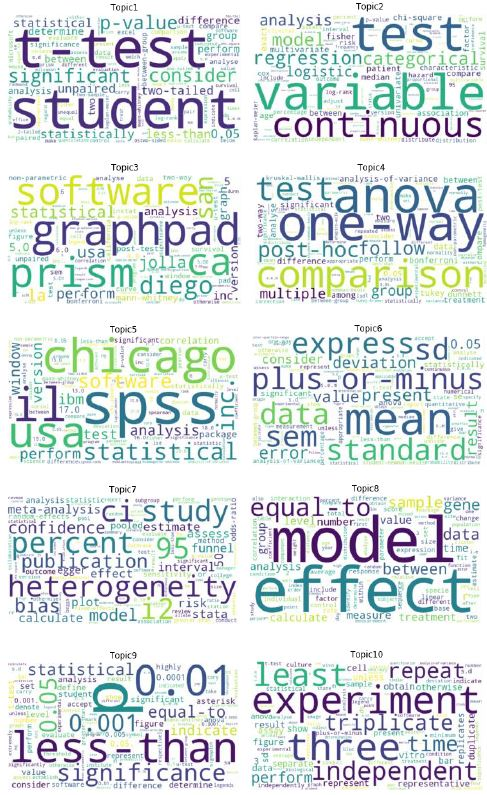
\includegraphics[width=0.8\linewidth]{figures/ploswordclouds} 

}

\caption{\label{fig:plos-clouds}Word clouds for ten topics for statistical methods sections published in PLOS ONE}\label{fig:unnamed-chunk-6}
\end{figure}

The word clouds for ten topics are in Figure \ref{fig:plos-clouds}.
Frequently occurring words reflected the use of statistical software
(topics 3 and 5), descriptive statistics (topic 6), group based
hypothesis testing (topics 1 and 4) and definitions of statistical
significance (topics 1 and 9). Topics related to
regression (topic 2) and meta-analysis (topic 7) were also identified.
Examples of boilerplate text for selected topics are in Table
\ref{tab:plos-example-boilerplate}.

Topics related to statistical software differentiated between Prism
GraphPad (topic 3: n = 9974) and SPSS (topic 5: n = 9648).
Within topic 3, the sentence ``GraphPad Prism (Graphpad Software, San
Diego, CA) was used for all analyses'' was matched in 1,941 papers based on our definition of boilerplate text.
Similarly, for topic 5, ``SPSS software version
17.0 (SPSS, Chicago, IL, USA) was used for statistical analysis'' returned matches for 441 papers.

\begin{landscape}
\begin{table}

\caption{\label{tab:plos-example-boilerplate}Example boilerplate text from PLOS ONE papers (sentence level). The number of matching to each sentence was based on a Jaccard score of 0.9 or higher and a difference in word count of $\pm$ 3 words}
\centering
\begin{tabular}[t]{p{0.1\textwidth}p{0.9\textwidth}p{0.1\textwidth}}
\hline
Topic & Statistical methods text & Matching papers\\
\hline
Topic 1 & Students t-test was used for statistical analysis. & 29\\
\cline{2-3}
 & A p value of $<$ 0.05 was considered statistically significant. & 1883\\
\hline
Topic 3 & GraphPad Prism (Graphpad Software, San Diego, CA) was used for all analyses. & 1941\\
\hline
Topic 4 & Significant differences were determined using analysis of variance (ANOVA) followed by tukey post-hoc tests for multiple comparisons. & 2216\\
\hline
Topic 5 & SPSS software version 17.0 (SPSS, Chicago, IL, USA) was used for statistical analysis. & 441\\
\hline
Topic 6 & All results are expressed as means $\pm$ standard deviation ($\pm$ SD). & 102\\
\hline
Topic 9 & Statistical significance was determined by Students t-tests. & 49\\
\cline{2-3}
&  $^*$p $<$ 0.05, $^{**}$p $<$ 0.01, $^{***}$p $<$ 0.001. & 6\\
\hline
\end{tabular}
\end{table}
\end{landscape}


Definitions of statistical significance featured strongly in topic 1 (n
= 3784) and topic 9 (n = 6195). Topic 1 reflected
applications of two-tailed and unpaired Student's t-tests, however,
instances of boilerplate text emphasised the 5\% level of statistical
significance (Table \ref{tab:plos-example-boilerplate}). In contrast, Topic 9
focused on multiple thresholds for declaring statistical significance by
asterisk: ``\(^{*}p<0.05\), \(^{**}p<0.01\) and \(^{***}p<0.001\)'', a
practice that has been criticised \citep{Wasserstein2019}.

Group-based hypothesis testing was a recurring theme across topics, with
text descriptions varying based on method(s) used. One-way analysis of
variance also featured strongly in topic 4 (n = 10212), combined
with common methods for performing post-hoc multiple comparisons. Based
on the Jaccard index, 1 in 5 studies were matched to the sentence
``Significant differences were determined using analysis of variance
(ANOVA) followed by Tukey post-hoc tests for multiple comparisons''.
Frequently occurring words in topic 6 (n = 4764) reflected
mentions of descriptive statistics for summarising continuous variables,
namely means with standard deviations or standard errors.

\subsection{ANZCTR}

We downloaded 28,008 studies. The numbers of excluded studies are shown
in Figure \ref{fig:consort-diagrams}. Of the 12,700 included studies,
9,523 (75\%) had a statistical methods section. The median length of
sections was 129 words with an inter-quartile range of 71 to 219 words.

Odds ratios and 95\% credible intervals for study characteristics
associated with missing statistical methods sections are in Table
\ref{tab:anzctr-missing-odds}. Observational studies were less likely to
have a missing statistical methods section compared with interventional
studies. Missing sections became less likely over time. Studies with
more funders and a larger target sample size were less likely to have a
missing statistical methods section.

\begin{table}[]
\centering
\caption{Logistic regression results for study characteristics associated with missing statistical methods sections in ANZCTR}
\label{tab:anzctr-missing-odds}
\begin{tabular}{lcc}
\hline
Variable & Odds ratio & 95$\%$ CI \\
\hline
Study type $=$ Observational & 0.78 & (0.69, 0.89) \\
Date (per year) & 0.90 & (0.88, 0.91) \\
Number of funders & 0.80 & (0.74, 0.86) \\
Target sample size (per doubling) & 0.90 & (0.88, 0.92)\\
\hline
\end{tabular}
\end{table}

\begin{figure}

{\centering 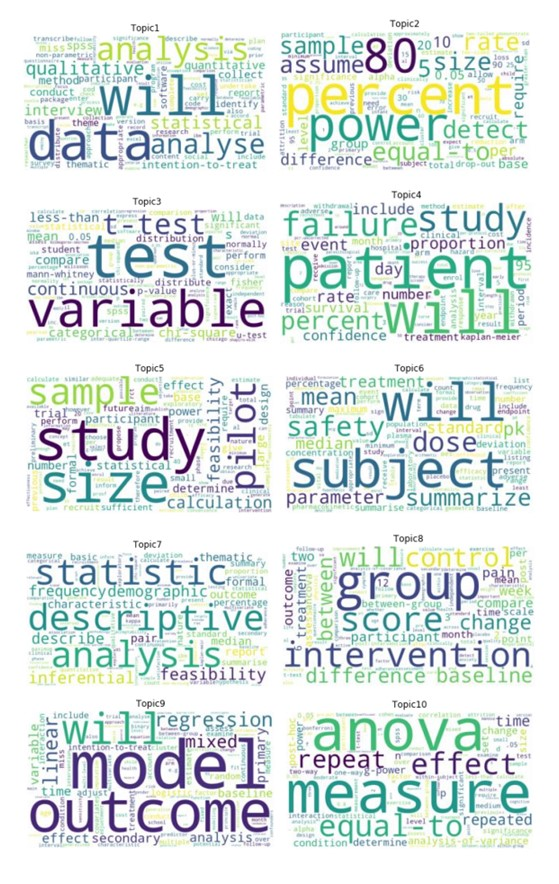
\includegraphics[width=0.7\linewidth]{figures/anzctrwordclouds} 

}

\caption{Word clouds for ten topics for statistical methods sections published in ANZCTR}\label{fig:unnamed-chunk-9}
\end{figure}

The text clustering algorithm found topics that were purely sample size
calculations (topic 2, n = 1834), pilot studies (topic 5, n = 834),
safety/tolerability studies (topic 6, n = 524), intervention studies
(topic 8, n = 1020) and repeated measures ANOVA (topic 10 = 852).
Examples of boilerplate text are provided in Table
\ref{tab:anzctr-example-boilerplate} .

Some methods sections were only one word, including ``ANOVA'',
``t-test'', ``SPSS'' and even ``SSPS''. There were cases where the exact
same method section had been re-used in a different study. For example,
in topic 7 (n = 333), 232 sections stated `descriptive statistics' or
`descriptive statistics used' with no additional details provided. Other
instances with expanded descriptions of methods included topic 3 (n =
1277) outlining descriptive analyses only, and topic 6 (n = 524), for
hypothesis testing methods, statistical significance and software. 
In other cases, text had been slightly modified to account for changes
in primary and secondary outcomes. Examples of these text changes were
found in topics 2 and 4; identified instances
related to sample size calculations for patient recruitment to different
studies.

Since studies in this dataset described planned analyses, we
hypothesised that some studies did not specify statistical methods because
they had yet to consult with a statistician. Targeted searches for ``statistician'' across all topics returned 1,277 matching studies,
with examples including ``A statistician employed by hospital was used''
and ``Pilot study at this point will use a statistician professionally
to determine sample size calculations as required''.

\begin{landscape}
\begin{table}[]
\centering
\caption{Example boilerplate text from ANZCTR dataset}
\label{tab:anzctr-example-boilerplate}
\begin{tabular}{p{0.1\linewidth} p{0.9\linewidth}}
\hline
\textbf{Topic} & \textbf{Statistical methods section} \\ \hline
3 & Comparisons between categorical variables will be made either using chi square or Fisher exact test. Continuous data will be compared using the Student’s t-test or Mann-Whitney U test. Two sided p values of less than 0.05 will be considered statistically significant.\\
 &  The Mann-Whitney U, Student t, 1-way ANOVA, and Kruskal-Wallis tests will be used to compare continuous variables where relevant. The Fisher exact and Pearson’s Chi-square test will be used to compare proportions as appropriate. \\ \hline
5 & Pilot study \\
 &  No formal sample size calculation was performed \\ \hline
7 & Descriptive statistics \\
 &  Descriptive statistics used \\ \hline
9 & Linear mixed models will be used to analyse the data. \\ \hline
10 & Repeated measures of ANOVA \\
 &  Pre-, during, post- and follow-up variables will be subjected to mixed methods and repeated measures analyses to determine significant changes over (group and) time. \\ \hline
\end{tabular}
\end{table}
\end{landscape}

\hypertarget{discussion}{%
\section{Discussion}\label{discussion}}

The first line in many statistical analysis sections in \emph{PLOS ONE}
was the software used and some entire sections in ANZCTR only stated the
software, implying that the software is the most important detail. As
Doug Altman said, ``Many people think that all you need to do statistics
is a computer and appropriate software'' \citep{Altman1994}. This is far
from the truth, and whilst it is important for researchers to mention
the software and version used for reproducibility purposes, it is a
minor detail compared with detailing what methods were used and why.

A frequent theme in the boilerplate statistical methods is the
definition of statistical significance, nearly always using a p-value at
the 5\% level. This widespread use of statistical significance is
troubling giving the bright-line thinking it engenders
\citep{McShane2019} and the common misinterpretations of p-values
\citep{Goodman2008}.

Despite the extensive array of statistical tests available, many authors
are reporting the same few methods.

One reason these inadequate sections get published is that most journals
do not use statistical reviewers, despite empirical evidence showing
they improve manuscript quality \citep{Hardwicke2020}.

A related paper has criticised vague statistical methods sections
because they deprive readers and reviewers for the opportunity to
confirm that the appropriate methods were used \citep{Weissgerber2018}.
These authors checked hundreds of papers using ANOVA and found that 95\%
did not contain the information needed to determine what type of ANOVA
was performed. This lack of information could well be because the
authors used a boilerplate statistical methods section that was missing
key details.

If authors shared their code then this would provide an alternative
route for checking what statistical methods were used. This is not a
perfect solution, as we still want authors to accurately report their
methods, but it does increase transparency. However, a recent paper
found that code sharing was very low in biomedical papers, with just 2\%
of a sample of over 6,000 papers sharing code \citep{Serghiou2021}.

Many researchers are using lazy practice by copying a standard
``boilerplate'' statistical methods section, likely cut-and-pasting from
other researchers or projects. This is a strong sign of the ritualistic
practice of statistics where researchers go through the motions rather
than using conscientious practice \citep{Stark2018}. This is concerning
because using the wrong statistical methods can reduce the value of
study, or worse, invalidate the entire study. These mistakes are
avoidable and are wasting of thousands of hours of researchers' time and
the time of patients and volunteers. Poor statistical practice is a key
driver of the ongoing reproducibility crisis in science
\citep{Ioannidis2014}.

\hypertarget{limitations}{%
\subsection{Limitations}\label{limitations}}

We did not check whether papers used the correct methods, and for some
simple studies a `boilerplate' statistical methods might be adequate.

We examined papers where there was a statistics section, and we missed
papers that used statistical analysis but did not include a statistical
analysis section. Reiterate outcomes of random sample checking here.

We only examined one large journal and one trial registry and hence our
results may not be generalisable to all journals or registries,
especially those that consistently use a statistical reviewer.

We searched the full text of \emph{PLOS ONE} papers but not the
supporting information which may contain statistical methods sections
for some papers. The search terms we used to find statistical methods
appeared in the supporting information titles for xxx papers (x\%). We
did not include the supporting information because it is less structured
than the paper and could be in PDF or Word format.

\bibliographystyle{agsm}
\bibliography{references}

\end{document}
